% **************************************************************************************************************
% A Classic Thesis Style
% An Homage to The Elements of Typographic Style
%
% Copyright (C) 2015 André Miede http://www.miede.de
%
% If you like the style then I would appreciate a postcard. My address 
% can be found in the file ClassicThesis.pdf. A collection of the 
% postcards I received so far is available online at 
% http://postcards.miede.de
%
% License:
% This program is free software; you can redistribute it and/or modify
% it under the terms of the GNU General Public License as published by
% the Free Software Foundation; either version 2 of the License, or
% (at your option) any later version.
%
% This program is distributed in the hope that it will be useful,
% but WITHOUT ANY WARRANTY; without even the implied warranty of
% MERCHANTABILITY or FITNESS FOR A PARTICULAR PURPOSE.  See the
% GNU General Public License for more details.
%
% You should have received a copy of the GNU General Public License
% along with this program; see the file COPYING.  If not, write to
% the Free Software Foundation, Inc., 59 Temple Place - Suite 330,
% Boston, MA 02111-1307, USA.
%
% **************************************************************************************************************
\RequirePackage{fix-cm} % fix some latex issues see: http://texdoc.net/texmf-dist/doc/latex/base/fixltx2e.pdf
\documentclass[ twoside,openright,titlepage,numbers=noenddot,headinclude,%1headlines,% letterpaper a4paper
                footinclude=true,cleardoublepage=empty,abstractoff, % <--- obsolete, remove (todo)
                BCOR=5mm,paper=a4,fontsize=11pt,%11pt,a4paper,%
                ngerman,american,%
                ]{scrreprt}

%********************************************************************
% Note: Make all your adjustments in here
%*******************************************************
% ****************************************************************************************************
% classicthesis-config.tex 
% formerly known as loadpackages.sty, classicthesis-ldpkg.sty, and classicthesis-preamble.sty 
% Use it at the beginning of your ClassicThesis.tex, or as a LaTeX Preamble 
% in your ClassicThesis.{tex,lyx} with % ****************************************************************************************************
% classicthesis-config.tex 
% formerly known as loadpackages.sty, classicthesis-ldpkg.sty, and classicthesis-preamble.sty 
% Use it at the beginning of your ClassicThesis.tex, or as a LaTeX Preamble 
% in your ClassicThesis.{tex,lyx} with % ****************************************************************************************************
% classicthesis-config.tex 
% formerly known as loadpackages.sty, classicthesis-ldpkg.sty, and classicthesis-preamble.sty 
% Use it at the beginning of your ClassicThesis.tex, or as a LaTeX Preamble 
% in your ClassicThesis.{tex,lyx} with \input{classicthesis-config}
% ****************************************************************************************************  
% If you like the classicthesis, then I would appreciate a postcard. 
% My address can be found in the file ClassicThesis.pdf. A collection 
% of the postcards I received so far is available online at 
% http://postcards.miede.de
% ****************************************************************************************************


% ****************************************************************************************************
% 0. Set the encoding of your files. UTF-8 is the only sensible encoding nowadays. If you can't read
% äöüßáéçèê∂åëæƒÏ€ then change the encoding setting in your editor, not the line below. If your editor
% does not support utf8 use another editor!
% ****************************************************************************************************
\PassOptionsToPackage{utf8}{inputenc}
	\usepackage{inputenc}


\newcommand*\justify{%
	\fontdimen2\font=0.4em% interword space
	\fontdimen3\font=0.2em% interword stretch
	\fontdimen4\font=0.1em% interword shrink
	\fontdimen7\font=0.1em% extra space
	\hyphenchar\font=`\-% allowing hyphenation
}

\usepackage{dirtree}


% ****************************************************************************************************
% 1. Configure classicthesis for your needs here, e.g., remove "drafting" below 
% in order to deactivate the time-stamp on the pages
% ****************************************************************************************************
\PassOptionsToPackage{eulerchapternumbers,listings,%drafting,%
					 pdfspacing,%floatperchapter,%linedheaders,%
					 subfig,beramono,eulermath,parts,
				 	 dottedtoc}{classicthesis}                                        
% ********************************************************************
% Available options for classicthesis.sty 
% (see ClassicThesis.pdf for more information):
% drafting
% parts nochapters linedheaders
% eulerchapternumbers beramono eulermath pdfspacing minionprospacing
% tocaligned dottedtoc manychapters
% listings floatperchapter subfig
% ********************************************************************



% ****************************************************************************************************
% 2. Personal data and user ad-hoc commands
% ****************************************************************************************************
\newcommand{\myTitle}{Integración de Idemix en entornos de IoT\xspace}
\newcommand{\mySubtitle}{}
\newcommand{\myDegree}{}%Doktor-Ingenieur (Dr.-Ing.)\xspace}
\newcommand{\myName}{José Luis Cánovas Sánchez\xspace}
\newcommand{\myProf}{Antonio Fernando Skarmeta Gómez\xspace}
\newcommand{\myOtherProf}{Jorge Bernal Bernabé\xspace}
\newcommand{\mySupervisor}{}%Put name here\xspace}
\newcommand{\myFaculty}{Facultad de Ingeniería Informática\xspace}
\newcommand{\myDepartment}{}%Put data here\xspace}
\newcommand{\myUni}{Universidad de Murcia\xspace}
\newcommand{\myLocation}{Murcia}%Saarbrücken\xspace}
\newcommand{\myTime}{Junio 2017}%September 2015\xspace}
\newcommand{\myVersion}{}%version 4.2\xspace}

% ********************************************************************
% Setup, finetuning, and useful commands
% ********************************************************************
\newcounter{dummy} % necessary for correct hyperlinks (to index, bib, etc.)
\newlength{\abcd} % for ab..z string length calculation
\providecommand{\mLyX}{L\kern-.1667em\lower.25em\hbox{Y}\kern-.125emX\@}
\newcommand{\ie}{i.\,e.}
\newcommand{\Ie}{I.\,e.}
\newcommand{\eg}{e.\,g.}
\newcommand{\Eg}{E.\,g.} 
% ****************************************************************************************************


% ****************************************************************************************************
% 3. Loading some handy packages
% ****************************************************************************************************
% ******************************************************************** 
% Packages with options that might require adjustments
% ******************************************************************** 
%\PassOptionsToPackage{ngerman,american}{babel}   % change this to your language(s)
% Spanish languages need extra options in order to work with this template
%\PassOptionsToPackage{spanish,es-lcroman}{babel}
	\usepackage{babel}                  

\usepackage{csquotes}
\PassOptionsToPackage{%
    %backend=biber, %instead of bibtex
	backend=bibtex8,bibencoding=ascii,%
	language=auto,%
	style=numeric-comp,%
    %style=authoryear-comp, % Author 1999, 2010
    %bibstyle=authoryear,dashed=false, % dashed: substitute rep. author with ---
    sorting=nyt, % name, year, title
    maxbibnames=10, % default: 3, et al.
    %backref=true,%
    natbib=true % natbib compatibility mode (\citep and \citet still work)
}{biblatex}
    \usepackage{biblatex}

\PassOptionsToPackage{fleqn}{amsmath}       % math environments and more by the AMS 
    \usepackage{amsmath}

% ******************************************************************** 
% General useful packages
% ******************************************************************** 
\PassOptionsToPackage{T1}{fontenc} % T2A for cyrillics
    \usepackage{fontenc}     
\usepackage{textcomp} % fix warning with missing font shapes
\usepackage{scrhack} % fix warnings when using KOMA with listings package          
\usepackage{xspace} % to get the spacing after macros right  
\usepackage{mparhack} % get marginpar right
\usepackage{fixltx2e} % fixes some LaTeX stuff --> since 2015 in the LaTeX kernel (see below)
%\usepackage[latest]{latexrelease} % will be used once available in more distributions (ISSUE #107)
\PassOptionsToPackage{printonlyused,smaller}{acronym} 
    \usepackage{acronym} % nice macros for handling all acronyms in the thesis
    %\renewcommand{\bflabel}[1]{{#1}\hfill} % fix the list of acronyms --> no longer working
    %\renewcommand*{\acsfont}[1]{\textsc{#1}} 
    \renewcommand*{\aclabelfont}[1]{\acsfont{#1}}
% ****************************************************************************************************


% ****************************************************************************************************
% 4. Setup floats: tables, (sub)figures, and captions
% ****************************************************************************************************
\usepackage{tabularx} % better tables
    \setlength{\extrarowheight}{3pt} % increase table row height
\newcommand{\tableheadline}[1]{\multicolumn{1}{c}{\spacedlowsmallcaps{#1}}}
\newcommand{\myfloatalign}{\centering} % to be used with each float for alignment
\usepackage{caption}
% Thanks to cgnieder and Claus Lahiri
% http://tex.stackexchange.com/questions/69349/spacedlowsmallcaps-in-caption-label
% [REMOVED DUE TO OTHER PROBLEMS, SEE ISSUE #82]    
%\DeclareCaptionLabelFormat{smallcaps}{\bothIfFirst{#1}{~}\MakeTextLowercase{\textsc{#2}}}
%\captionsetup{font=small,labelformat=smallcaps} % format=hang,
\captionsetup{font=small} % format=hang,
\usepackage{subfig}  
% ****************************************************************************************************


% ****************************************************************************************************
% 5. Setup code listings
% ****************************************************************************************************
\usepackage{listings} 
%\lstset{emph={trueIndex,root},emphstyle=\color{BlueViolet}}%\underbar} % for special keywords
\lstset{language=[LaTeX]Tex,%C++,
    morekeywords={PassOptionsToPackage,selectlanguage},
    keywordstyle=\color{RoyalBlue},%\bfseries,
    basicstyle=\small\ttfamily,
    %identifierstyle=\color{NavyBlue},
    commentstyle=\color{Green}\ttfamily,
    stringstyle=\rmfamily,
    numbers=none,%left,%
    numberstyle=\scriptsize,%\tiny
    stepnumber=5,
    numbersep=8pt,
    showstringspaces=false,
    breaklines=true,
    %frameround=ftff,
    %frame=single,
    belowcaptionskip=.75\baselineskip
    %frame=L
} 
% ****************************************************************************************************             


% ****************************************************************************************************
% 6. PDFLaTeX, hyperreferences and citation backreferences
% ****************************************************************************************************
% ********************************************************************
% Using PDFLaTeX
% ********************************************************************
\PassOptionsToPackage{pdftex,hyperfootnotes=false,pdfpagelabels}{hyperref}
    \usepackage{hyperref}  % backref linktocpage pagebackref
\pdfcompresslevel=9
\pdfadjustspacing=1 
\PassOptionsToPackage{pdftex}{graphicx}
    \usepackage{graphicx} 
 

% ********************************************************************
% Hyperreferences
% ********************************************************************
\hypersetup{%
    %draft, % = no hyperlinking at all (useful in b/w printouts)
    colorlinks=true, linktocpage=true, pdfstartpage=1, pdfstartview=FitV,%
    % uncomment the following line if you want to have black links (e.g., for printing)
    %colorlinks=false, linktocpage=false, pdfstartpage=3, pdfstartview=FitV, pdfborder={0 0 0},%
    breaklinks=true, pdfpagemode=UseNone, pageanchor=true, pdfpagemode=UseOutlines,%
    plainpages=false, bookmarksnumbered, bookmarksopen=true, bookmarksopenlevel=1,%
    hypertexnames=true, pdfhighlight=/O,%nesting=true,%frenchlinks,%
    urlcolor=webbrown, linkcolor=RoyalBlue, citecolor=webgreen, %pagecolor=RoyalBlue,%
    %urlcolor=Black, linkcolor=Black, citecolor=Black, %pagecolor=Black,%
    pdftitle={\myTitle},%
    pdfauthor={\textcopyright\ \myName, \myUni, \myFaculty},%
    pdfsubject={},%
    pdfkeywords={},%
    pdfcreator={pdfLaTeX},%
    pdfproducer={LaTeX with hyperref and classicthesis}%
}   

% ********************************************************************
% Setup autoreferences
% ********************************************************************
% There are some issues regarding autorefnames
% http://www.ureader.de/msg/136221647.aspx
% http://www.tex.ac.uk/cgi-bin/texfaq2html?label=latexwords
% you have to redefine the makros for the 
% language you use, e.g., american, ngerman
% (as chosen when loading babel/AtBeginDocument)
% ********************************************************************
\makeatletter
\@ifpackageloaded{babel}%
    {%
       \addto\extrasamerican{%
			\renewcommand*{\figureautorefname}{Figure}%
			\renewcommand*{\tableautorefname}{Table}%
			\renewcommand*{\partautorefname}{Part}%
			\renewcommand*{\chapterautorefname}{Chapter}%
			\renewcommand*{\sectionautorefname}{Section}%
			\renewcommand*{\subsectionautorefname}{Section}%
			\renewcommand*{\subsubsectionautorefname}{Section}%     
                }%
       \addto\extrasngerman{% 
			\renewcommand*{\paragraphautorefname}{Absatz}%
			\renewcommand*{\subparagraphautorefname}{Unterabsatz}%
			\renewcommand*{\footnoteautorefname}{Fu\"snote}%
			\renewcommand*{\FancyVerbLineautorefname}{Zeile}%
			\renewcommand*{\theoremautorefname}{Theorem}%
			\renewcommand*{\appendixautorefname}{Anhang}%
			\renewcommand*{\equationautorefname}{Gleichung}%        
			\renewcommand*{\itemautorefname}{Punkt}%
                }%  
            % Fix to getting autorefs for subfigures right (thanks to Belinda Vogt for changing the definition)
            \providecommand{\subfigureautorefname}{\figureautorefname}%             
    }{\relax}
\makeatother


% ****************************************************************************************************
% 7. Last calls before the bar closes
% ****************************************************************************************************
% ********************************************************************
% Development Stuff
% ********************************************************************
\listfiles
%\PassOptionsToPackage{l2tabu,orthodox,abort}{nag}
%   \usepackage{nag}
%\PassOptionsToPackage{warning, all}{onlyamsmath}
%   \usepackage{onlyamsmath}

% ********************************************************************
% Last, but not least...
% ********************************************************************
\usepackage{classicthesis} 
% ****************************************************************************************************


% ****************************************************************************************************
% 8. Further adjustments (experimental)
% ****************************************************************************************************
% ********************************************************************
% Changing the text area
% ********************************************************************
\linespread{1.05} % a bit more for Palatino
%\areaset[current]{312pt}{761pt} % 686 (factor 2.2) + 33 head + 42 head \the\footskip
%\setlength{\marginparwidth}{7em}%
%\setlength{\marginparsep}{2em}%

% ********************************************************************
% Using different fonts
% ********************************************************************
%\usepackage[oldstylenums]{kpfonts} % oldstyle notextcomp
%\usepackage[osf]{libertine}
%\usepackage[light,condensed,math]{iwona}
%\renewcommand{\sfdefault}{iwona}
%\usepackage{lmodern} % <-- no osf support :-(
%\usepackage{cfr-lm} % 
%\usepackage[urw-garamond]{mathdesign} <-- no osf support :-(
%\usepackage[default,osfigures]{opensans} % scale=0.95 
%\usepackage[sfdefault]{FiraSans}
% ****************************************************************************************************

% ****************************************************************************************************  
% If you like the classicthesis, then I would appreciate a postcard. 
% My address can be found in the file ClassicThesis.pdf. A collection 
% of the postcards I received so far is available online at 
% http://postcards.miede.de
% ****************************************************************************************************


% ****************************************************************************************************
% 0. Set the encoding of your files. UTF-8 is the only sensible encoding nowadays. If you can't read
% äöüßáéçèê∂åëæƒÏ€ then change the encoding setting in your editor, not the line below. If your editor
% does not support utf8 use another editor!
% ****************************************************************************************************
\PassOptionsToPackage{utf8}{inputenc}
	\usepackage{inputenc}


\newcommand*\justify{%
	\fontdimen2\font=0.4em% interword space
	\fontdimen3\font=0.2em% interword stretch
	\fontdimen4\font=0.1em% interword shrink
	\fontdimen7\font=0.1em% extra space
	\hyphenchar\font=`\-% allowing hyphenation
}

\usepackage{dirtree}


% ****************************************************************************************************
% 1. Configure classicthesis for your needs here, e.g., remove "drafting" below 
% in order to deactivate the time-stamp on the pages
% ****************************************************************************************************
\PassOptionsToPackage{eulerchapternumbers,listings,%drafting,%
					 pdfspacing,%floatperchapter,%linedheaders,%
					 subfig,beramono,eulermath,parts,
				 	 dottedtoc}{classicthesis}                                        
% ********************************************************************
% Available options for classicthesis.sty 
% (see ClassicThesis.pdf for more information):
% drafting
% parts nochapters linedheaders
% eulerchapternumbers beramono eulermath pdfspacing minionprospacing
% tocaligned dottedtoc manychapters
% listings floatperchapter subfig
% ********************************************************************



% ****************************************************************************************************
% 2. Personal data and user ad-hoc commands
% ****************************************************************************************************
\newcommand{\myTitle}{Integración de Idemix en entornos de IoT\xspace}
\newcommand{\mySubtitle}{}
\newcommand{\myDegree}{}%Doktor-Ingenieur (Dr.-Ing.)\xspace}
\newcommand{\myName}{José Luis Cánovas Sánchez\xspace}
\newcommand{\myProf}{Antonio Fernando Skarmeta Gómez\xspace}
\newcommand{\myOtherProf}{Jorge Bernal Bernabé\xspace}
\newcommand{\mySupervisor}{}%Put name here\xspace}
\newcommand{\myFaculty}{Facultad de Ingeniería Informática\xspace}
\newcommand{\myDepartment}{}%Put data here\xspace}
\newcommand{\myUni}{Universidad de Murcia\xspace}
\newcommand{\myLocation}{Murcia}%Saarbrücken\xspace}
\newcommand{\myTime}{Junio 2017}%September 2015\xspace}
\newcommand{\myVersion}{}%version 4.2\xspace}

% ********************************************************************
% Setup, finetuning, and useful commands
% ********************************************************************
\newcounter{dummy} % necessary for correct hyperlinks (to index, bib, etc.)
\newlength{\abcd} % for ab..z string length calculation
\providecommand{\mLyX}{L\kern-.1667em\lower.25em\hbox{Y}\kern-.125emX\@}
\newcommand{\ie}{i.\,e.}
\newcommand{\Ie}{I.\,e.}
\newcommand{\eg}{e.\,g.}
\newcommand{\Eg}{E.\,g.} 
% ****************************************************************************************************


% ****************************************************************************************************
% 3. Loading some handy packages
% ****************************************************************************************************
% ******************************************************************** 
% Packages with options that might require adjustments
% ******************************************************************** 
%\PassOptionsToPackage{ngerman,american}{babel}   % change this to your language(s)
% Spanish languages need extra options in order to work with this template
%\PassOptionsToPackage{spanish,es-lcroman}{babel}
	\usepackage{babel}                  

\usepackage{csquotes}
\PassOptionsToPackage{%
    %backend=biber, %instead of bibtex
	backend=bibtex8,bibencoding=ascii,%
	language=auto,%
	style=numeric-comp,%
    %style=authoryear-comp, % Author 1999, 2010
    %bibstyle=authoryear,dashed=false, % dashed: substitute rep. author with ---
    sorting=nyt, % name, year, title
    maxbibnames=10, % default: 3, et al.
    %backref=true,%
    natbib=true % natbib compatibility mode (\citep and \citet still work)
}{biblatex}
    \usepackage{biblatex}

\PassOptionsToPackage{fleqn}{amsmath}       % math environments and more by the AMS 
    \usepackage{amsmath}

% ******************************************************************** 
% General useful packages
% ******************************************************************** 
\PassOptionsToPackage{T1}{fontenc} % T2A for cyrillics
    \usepackage{fontenc}     
\usepackage{textcomp} % fix warning with missing font shapes
\usepackage{scrhack} % fix warnings when using KOMA with listings package          
\usepackage{xspace} % to get the spacing after macros right  
\usepackage{mparhack} % get marginpar right
\usepackage{fixltx2e} % fixes some LaTeX stuff --> since 2015 in the LaTeX kernel (see below)
%\usepackage[latest]{latexrelease} % will be used once available in more distributions (ISSUE #107)
\PassOptionsToPackage{printonlyused,smaller}{acronym} 
    \usepackage{acronym} % nice macros for handling all acronyms in the thesis
    %\renewcommand{\bflabel}[1]{{#1}\hfill} % fix the list of acronyms --> no longer working
    %\renewcommand*{\acsfont}[1]{\textsc{#1}} 
    \renewcommand*{\aclabelfont}[1]{\acsfont{#1}}
% ****************************************************************************************************


% ****************************************************************************************************
% 4. Setup floats: tables, (sub)figures, and captions
% ****************************************************************************************************
\usepackage{tabularx} % better tables
    \setlength{\extrarowheight}{3pt} % increase table row height
\newcommand{\tableheadline}[1]{\multicolumn{1}{c}{\spacedlowsmallcaps{#1}}}
\newcommand{\myfloatalign}{\centering} % to be used with each float for alignment
\usepackage{caption}
% Thanks to cgnieder and Claus Lahiri
% http://tex.stackexchange.com/questions/69349/spacedlowsmallcaps-in-caption-label
% [REMOVED DUE TO OTHER PROBLEMS, SEE ISSUE #82]    
%\DeclareCaptionLabelFormat{smallcaps}{\bothIfFirst{#1}{~}\MakeTextLowercase{\textsc{#2}}}
%\captionsetup{font=small,labelformat=smallcaps} % format=hang,
\captionsetup{font=small} % format=hang,
\usepackage{subfig}  
% ****************************************************************************************************


% ****************************************************************************************************
% 5. Setup code listings
% ****************************************************************************************************
\usepackage{listings} 
%\lstset{emph={trueIndex,root},emphstyle=\color{BlueViolet}}%\underbar} % for special keywords
\lstset{language=[LaTeX]Tex,%C++,
    morekeywords={PassOptionsToPackage,selectlanguage},
    keywordstyle=\color{RoyalBlue},%\bfseries,
    basicstyle=\small\ttfamily,
    %identifierstyle=\color{NavyBlue},
    commentstyle=\color{Green}\ttfamily,
    stringstyle=\rmfamily,
    numbers=none,%left,%
    numberstyle=\scriptsize,%\tiny
    stepnumber=5,
    numbersep=8pt,
    showstringspaces=false,
    breaklines=true,
    %frameround=ftff,
    %frame=single,
    belowcaptionskip=.75\baselineskip
    %frame=L
} 
% ****************************************************************************************************             


% ****************************************************************************************************
% 6. PDFLaTeX, hyperreferences and citation backreferences
% ****************************************************************************************************
% ********************************************************************
% Using PDFLaTeX
% ********************************************************************
\PassOptionsToPackage{pdftex,hyperfootnotes=false,pdfpagelabels}{hyperref}
    \usepackage{hyperref}  % backref linktocpage pagebackref
\pdfcompresslevel=9
\pdfadjustspacing=1 
\PassOptionsToPackage{pdftex}{graphicx}
    \usepackage{graphicx} 
 

% ********************************************************************
% Hyperreferences
% ********************************************************************
\hypersetup{%
    %draft, % = no hyperlinking at all (useful in b/w printouts)
    colorlinks=true, linktocpage=true, pdfstartpage=1, pdfstartview=FitV,%
    % uncomment the following line if you want to have black links (e.g., for printing)
    %colorlinks=false, linktocpage=false, pdfstartpage=3, pdfstartview=FitV, pdfborder={0 0 0},%
    breaklinks=true, pdfpagemode=UseNone, pageanchor=true, pdfpagemode=UseOutlines,%
    plainpages=false, bookmarksnumbered, bookmarksopen=true, bookmarksopenlevel=1,%
    hypertexnames=true, pdfhighlight=/O,%nesting=true,%frenchlinks,%
    urlcolor=webbrown, linkcolor=RoyalBlue, citecolor=webgreen, %pagecolor=RoyalBlue,%
    %urlcolor=Black, linkcolor=Black, citecolor=Black, %pagecolor=Black,%
    pdftitle={\myTitle},%
    pdfauthor={\textcopyright\ \myName, \myUni, \myFaculty},%
    pdfsubject={},%
    pdfkeywords={},%
    pdfcreator={pdfLaTeX},%
    pdfproducer={LaTeX with hyperref and classicthesis}%
}   

% ********************************************************************
% Setup autoreferences
% ********************************************************************
% There are some issues regarding autorefnames
% http://www.ureader.de/msg/136221647.aspx
% http://www.tex.ac.uk/cgi-bin/texfaq2html?label=latexwords
% you have to redefine the makros for the 
% language you use, e.g., american, ngerman
% (as chosen when loading babel/AtBeginDocument)
% ********************************************************************
\makeatletter
\@ifpackageloaded{babel}%
    {%
       \addto\extrasamerican{%
			\renewcommand*{\figureautorefname}{Figure}%
			\renewcommand*{\tableautorefname}{Table}%
			\renewcommand*{\partautorefname}{Part}%
			\renewcommand*{\chapterautorefname}{Chapter}%
			\renewcommand*{\sectionautorefname}{Section}%
			\renewcommand*{\subsectionautorefname}{Section}%
			\renewcommand*{\subsubsectionautorefname}{Section}%     
                }%
       \addto\extrasngerman{% 
			\renewcommand*{\paragraphautorefname}{Absatz}%
			\renewcommand*{\subparagraphautorefname}{Unterabsatz}%
			\renewcommand*{\footnoteautorefname}{Fu\"snote}%
			\renewcommand*{\FancyVerbLineautorefname}{Zeile}%
			\renewcommand*{\theoremautorefname}{Theorem}%
			\renewcommand*{\appendixautorefname}{Anhang}%
			\renewcommand*{\equationautorefname}{Gleichung}%        
			\renewcommand*{\itemautorefname}{Punkt}%
                }%  
            % Fix to getting autorefs for subfigures right (thanks to Belinda Vogt for changing the definition)
            \providecommand{\subfigureautorefname}{\figureautorefname}%             
    }{\relax}
\makeatother


% ****************************************************************************************************
% 7. Last calls before the bar closes
% ****************************************************************************************************
% ********************************************************************
% Development Stuff
% ********************************************************************
\listfiles
%\PassOptionsToPackage{l2tabu,orthodox,abort}{nag}
%   \usepackage{nag}
%\PassOptionsToPackage{warning, all}{onlyamsmath}
%   \usepackage{onlyamsmath}

% ********************************************************************
% Last, but not least...
% ********************************************************************
\usepackage{classicthesis} 
% ****************************************************************************************************


% ****************************************************************************************************
% 8. Further adjustments (experimental)
% ****************************************************************************************************
% ********************************************************************
% Changing the text area
% ********************************************************************
\linespread{1.05} % a bit more for Palatino
%\areaset[current]{312pt}{761pt} % 686 (factor 2.2) + 33 head + 42 head \the\footskip
%\setlength{\marginparwidth}{7em}%
%\setlength{\marginparsep}{2em}%

% ********************************************************************
% Using different fonts
% ********************************************************************
%\usepackage[oldstylenums]{kpfonts} % oldstyle notextcomp
%\usepackage[osf]{libertine}
%\usepackage[light,condensed,math]{iwona}
%\renewcommand{\sfdefault}{iwona}
%\usepackage{lmodern} % <-- no osf support :-(
%\usepackage{cfr-lm} % 
%\usepackage[urw-garamond]{mathdesign} <-- no osf support :-(
%\usepackage[default,osfigures]{opensans} % scale=0.95 
%\usepackage[sfdefault]{FiraSans}
% ****************************************************************************************************

% ****************************************************************************************************  
% If you like the classicthesis, then I would appreciate a postcard. 
% My address can be found in the file ClassicThesis.pdf. A collection 
% of the postcards I received so far is available online at 
% http://postcards.miede.de
% ****************************************************************************************************


% ****************************************************************************************************
% 0. Set the encoding of your files. UTF-8 is the only sensible encoding nowadays. If you can't read
% äöüßáéçèê∂åëæƒÏ€ then change the encoding setting in your editor, not the line below. If your editor
% does not support utf8 use another editor!
% ****************************************************************************************************
\PassOptionsToPackage{utf8}{inputenc}
	\usepackage{inputenc}


\newcommand*\justify{%
	\fontdimen2\font=0.4em% interword space
	\fontdimen3\font=0.2em% interword stretch
	\fontdimen4\font=0.1em% interword shrink
	\fontdimen7\font=0.1em% extra space
	\hyphenchar\font=`\-% allowing hyphenation
}

\usepackage{dirtree}


% ****************************************************************************************************
% 1. Configure classicthesis for your needs here, e.g., remove "drafting" below 
% in order to deactivate the time-stamp on the pages
% ****************************************************************************************************
\PassOptionsToPackage{eulerchapternumbers,listings,%drafting,%
					 pdfspacing,%floatperchapter,%linedheaders,%
					 subfig,beramono,eulermath,parts,
				 	 dottedtoc}{classicthesis}                                        
% ********************************************************************
% Available options for classicthesis.sty 
% (see ClassicThesis.pdf for more information):
% drafting
% parts nochapters linedheaders
% eulerchapternumbers beramono eulermath pdfspacing minionprospacing
% tocaligned dottedtoc manychapters
% listings floatperchapter subfig
% ********************************************************************



% ****************************************************************************************************
% 2. Personal data and user ad-hoc commands
% ****************************************************************************************************
\newcommand{\myTitle}{Integración de Idemix en entornos de IoT\xspace}
\newcommand{\mySubtitle}{}
\newcommand{\myDegree}{}%Doktor-Ingenieur (Dr.-Ing.)\xspace}
\newcommand{\myName}{José Luis Cánovas Sánchez\xspace}
\newcommand{\myProf}{Antonio Fernando Skarmeta Gómez\xspace}
\newcommand{\myOtherProf}{Jorge Bernal Bernabé\xspace}
\newcommand{\mySupervisor}{}%Put name here\xspace}
\newcommand{\myFaculty}{Facultad de Ingeniería Informática\xspace}
\newcommand{\myDepartment}{}%Put data here\xspace}
\newcommand{\myUni}{Universidad de Murcia\xspace}
\newcommand{\myLocation}{Murcia}%Saarbrücken\xspace}
\newcommand{\myTime}{Junio 2017}%September 2015\xspace}
\newcommand{\myVersion}{}%version 4.2\xspace}

% ********************************************************************
% Setup, finetuning, and useful commands
% ********************************************************************
\newcounter{dummy} % necessary for correct hyperlinks (to index, bib, etc.)
\newlength{\abcd} % for ab..z string length calculation
\providecommand{\mLyX}{L\kern-.1667em\lower.25em\hbox{Y}\kern-.125emX\@}
\newcommand{\ie}{i.\,e.}
\newcommand{\Ie}{I.\,e.}
\newcommand{\eg}{e.\,g.}
\newcommand{\Eg}{E.\,g.} 
% ****************************************************************************************************


% ****************************************************************************************************
% 3. Loading some handy packages
% ****************************************************************************************************
% ******************************************************************** 
% Packages with options that might require adjustments
% ******************************************************************** 
%\PassOptionsToPackage{ngerman,american}{babel}   % change this to your language(s)
% Spanish languages need extra options in order to work with this template
%\PassOptionsToPackage{spanish,es-lcroman}{babel}
	\usepackage{babel}                  

\usepackage{csquotes}
\PassOptionsToPackage{%
    %backend=biber, %instead of bibtex
	backend=bibtex8,bibencoding=ascii,%
	language=auto,%
	style=numeric-comp,%
    %style=authoryear-comp, % Author 1999, 2010
    %bibstyle=authoryear,dashed=false, % dashed: substitute rep. author with ---
    sorting=nyt, % name, year, title
    maxbibnames=10, % default: 3, et al.
    %backref=true,%
    natbib=true % natbib compatibility mode (\citep and \citet still work)
}{biblatex}
    \usepackage{biblatex}

\PassOptionsToPackage{fleqn}{amsmath}       % math environments and more by the AMS 
    \usepackage{amsmath}

% ******************************************************************** 
% General useful packages
% ******************************************************************** 
\PassOptionsToPackage{T1}{fontenc} % T2A for cyrillics
    \usepackage{fontenc}     
\usepackage{textcomp} % fix warning with missing font shapes
\usepackage{scrhack} % fix warnings when using KOMA with listings package          
\usepackage{xspace} % to get the spacing after macros right  
\usepackage{mparhack} % get marginpar right
\usepackage{fixltx2e} % fixes some LaTeX stuff --> since 2015 in the LaTeX kernel (see below)
%\usepackage[latest]{latexrelease} % will be used once available in more distributions (ISSUE #107)
\PassOptionsToPackage{printonlyused,smaller}{acronym} 
    \usepackage{acronym} % nice macros for handling all acronyms in the thesis
    %\renewcommand{\bflabel}[1]{{#1}\hfill} % fix the list of acronyms --> no longer working
    %\renewcommand*{\acsfont}[1]{\textsc{#1}} 
    \renewcommand*{\aclabelfont}[1]{\acsfont{#1}}
% ****************************************************************************************************


% ****************************************************************************************************
% 4. Setup floats: tables, (sub)figures, and captions
% ****************************************************************************************************
\usepackage{tabularx} % better tables
    \setlength{\extrarowheight}{3pt} % increase table row height
\newcommand{\tableheadline}[1]{\multicolumn{1}{c}{\spacedlowsmallcaps{#1}}}
\newcommand{\myfloatalign}{\centering} % to be used with each float for alignment
\usepackage{caption}
% Thanks to cgnieder and Claus Lahiri
% http://tex.stackexchange.com/questions/69349/spacedlowsmallcaps-in-caption-label
% [REMOVED DUE TO OTHER PROBLEMS, SEE ISSUE #82]    
%\DeclareCaptionLabelFormat{smallcaps}{\bothIfFirst{#1}{~}\MakeTextLowercase{\textsc{#2}}}
%\captionsetup{font=small,labelformat=smallcaps} % format=hang,
\captionsetup{font=small} % format=hang,
\usepackage{subfig}  
% ****************************************************************************************************


% ****************************************************************************************************
% 5. Setup code listings
% ****************************************************************************************************
\usepackage{listings} 
%\lstset{emph={trueIndex,root},emphstyle=\color{BlueViolet}}%\underbar} % for special keywords
\lstset{language=[LaTeX]Tex,%C++,
    morekeywords={PassOptionsToPackage,selectlanguage},
    keywordstyle=\color{RoyalBlue},%\bfseries,
    basicstyle=\small\ttfamily,
    %identifierstyle=\color{NavyBlue},
    commentstyle=\color{Green}\ttfamily,
    stringstyle=\rmfamily,
    numbers=none,%left,%
    numberstyle=\scriptsize,%\tiny
    stepnumber=5,
    numbersep=8pt,
    showstringspaces=false,
    breaklines=true,
    %frameround=ftff,
    %frame=single,
    belowcaptionskip=.75\baselineskip
    %frame=L
} 
% ****************************************************************************************************             


% ****************************************************************************************************
% 6. PDFLaTeX, hyperreferences and citation backreferences
% ****************************************************************************************************
% ********************************************************************
% Using PDFLaTeX
% ********************************************************************
\PassOptionsToPackage{pdftex,hyperfootnotes=false,pdfpagelabels}{hyperref}
    \usepackage{hyperref}  % backref linktocpage pagebackref
\pdfcompresslevel=9
\pdfadjustspacing=1 
\PassOptionsToPackage{pdftex}{graphicx}
    \usepackage{graphicx} 
 

% ********************************************************************
% Hyperreferences
% ********************************************************************
\hypersetup{%
    %draft, % = no hyperlinking at all (useful in b/w printouts)
    colorlinks=true, linktocpage=true, pdfstartpage=1, pdfstartview=FitV,%
    % uncomment the following line if you want to have black links (e.g., for printing)
    %colorlinks=false, linktocpage=false, pdfstartpage=3, pdfstartview=FitV, pdfborder={0 0 0},%
    breaklinks=true, pdfpagemode=UseNone, pageanchor=true, pdfpagemode=UseOutlines,%
    plainpages=false, bookmarksnumbered, bookmarksopen=true, bookmarksopenlevel=1,%
    hypertexnames=true, pdfhighlight=/O,%nesting=true,%frenchlinks,%
    urlcolor=webbrown, linkcolor=RoyalBlue, citecolor=webgreen, %pagecolor=RoyalBlue,%
    %urlcolor=Black, linkcolor=Black, citecolor=Black, %pagecolor=Black,%
    pdftitle={\myTitle},%
    pdfauthor={\textcopyright\ \myName, \myUni, \myFaculty},%
    pdfsubject={},%
    pdfkeywords={},%
    pdfcreator={pdfLaTeX},%
    pdfproducer={LaTeX with hyperref and classicthesis}%
}   

% ********************************************************************
% Setup autoreferences
% ********************************************************************
% There are some issues regarding autorefnames
% http://www.ureader.de/msg/136221647.aspx
% http://www.tex.ac.uk/cgi-bin/texfaq2html?label=latexwords
% you have to redefine the makros for the 
% language you use, e.g., american, ngerman
% (as chosen when loading babel/AtBeginDocument)
% ********************************************************************
\makeatletter
\@ifpackageloaded{babel}%
    {%
       \addto\extrasamerican{%
			\renewcommand*{\figureautorefname}{Figure}%
			\renewcommand*{\tableautorefname}{Table}%
			\renewcommand*{\partautorefname}{Part}%
			\renewcommand*{\chapterautorefname}{Chapter}%
			\renewcommand*{\sectionautorefname}{Section}%
			\renewcommand*{\subsectionautorefname}{Section}%
			\renewcommand*{\subsubsectionautorefname}{Section}%     
                }%
       \addto\extrasngerman{% 
			\renewcommand*{\paragraphautorefname}{Absatz}%
			\renewcommand*{\subparagraphautorefname}{Unterabsatz}%
			\renewcommand*{\footnoteautorefname}{Fu\"snote}%
			\renewcommand*{\FancyVerbLineautorefname}{Zeile}%
			\renewcommand*{\theoremautorefname}{Theorem}%
			\renewcommand*{\appendixautorefname}{Anhang}%
			\renewcommand*{\equationautorefname}{Gleichung}%        
			\renewcommand*{\itemautorefname}{Punkt}%
                }%  
            % Fix to getting autorefs for subfigures right (thanks to Belinda Vogt for changing the definition)
            \providecommand{\subfigureautorefname}{\figureautorefname}%             
    }{\relax}
\makeatother


% ****************************************************************************************************
% 7. Last calls before the bar closes
% ****************************************************************************************************
% ********************************************************************
% Development Stuff
% ********************************************************************
\listfiles
%\PassOptionsToPackage{l2tabu,orthodox,abort}{nag}
%   \usepackage{nag}
%\PassOptionsToPackage{warning, all}{onlyamsmath}
%   \usepackage{onlyamsmath}

% ********************************************************************
% Last, but not least...
% ********************************************************************
\usepackage{classicthesis} 
% ****************************************************************************************************


% ****************************************************************************************************
% 8. Further adjustments (experimental)
% ****************************************************************************************************
% ********************************************************************
% Changing the text area
% ********************************************************************
\linespread{1.05} % a bit more for Palatino
%\areaset[current]{312pt}{761pt} % 686 (factor 2.2) + 33 head + 42 head \the\footskip
%\setlength{\marginparwidth}{7em}%
%\setlength{\marginparsep}{2em}%

% ********************************************************************
% Using different fonts
% ********************************************************************
%\usepackage[oldstylenums]{kpfonts} % oldstyle notextcomp
%\usepackage[osf]{libertine}
%\usepackage[light,condensed,math]{iwona}
%\renewcommand{\sfdefault}{iwona}
%\usepackage{lmodern} % <-- no osf support :-(
%\usepackage{cfr-lm} % 
%\usepackage[urw-garamond]{mathdesign} <-- no osf support :-(
%\usepackage[default,osfigures]{opensans} % scale=0.95 
%\usepackage[sfdefault]{FiraSans}
% ****************************************************************************************************


%********************************************************************
% Bibliographies
%*******************************************************
\addbibresource{Bibliography.bib}
%\addbibresource[label=ownpubs]{AMiede_Publications.bib}

%********************************************************************
% Hyphenation
%*******************************************************
%\hyphenation{put special hyphenation here}

% ********************************************************************
% GO!GO!GO! MOVE IT!
%*******************************************************
\begin{document}
\frenchspacing
\raggedbottom
\selectlanguage{american} % american ngerman
%\renewcommand*{\bibname}{new name}
%\setbibpreamble{}
\pagenumbering{roman}
\pagestyle{plain}
%********************************************************************
% Frontmatter
%*******************************************************
%%*******************************************************
% Little Dirty Titlepage
%*******************************************************
\thispagestyle{empty}
%\pdfbookmark[1]{Titel}{title}
%*******************************************************
\begin{center}
    \spacedlowsmallcaps{\myName} \\ \medskip                        

    \begingroup
        \color{Maroon}\spacedallcaps{\myTitle}
    \endgroup
\end{center}        

%*******************************************************
% Titlepage
%*******************************************************
\begin{titlepage}
    % if you want the titlepage to be centered, uncomment and fine-tune the line below (KOMA classes environment)
    \begin{addmargin}[-1cm]{-3cm}
    \begin{center}
        \large  

        \hfill

        \vfill

        \begingroup
            \color{Maroon}\spacedallcaps{\myTitle} \\ \bigskip
        \endgroup

        \spacedlowsmallcaps{\myName}
        
        \hfill
        
        Tutores
        
        \spacedlowsmallcaps{\myProf}

        \spacedlowsmallcaps{\myOtherProf}
        

        \vfill

        
\includegraphics[width=6cm]{gfx/ESCUDO} \\ \medskip

        %\mySubtitle \\ \medskip   
        %\myDegree \\
        %\myDepartment \\                            
        \myFaculty \\
        \myUni \\ \bigskip

        % \myTime\ -- \myVersion

        \vfill                      

    \end{center}  
  \end{addmargin}       
\end{titlepage}   
\thispagestyle{empty}

\hfill

\vfill

\noindent\myName: \textit{\myTitle}%,} %\mySubtitle, %\myDegree, \textcopyright\ \myTime

\bigskip
%
%\noindent\spacedlowsmallcaps{Tutores}: \\
%\myProf \\
%\myOtherProf \\ 
%\mySupervisor
%
%\medskip
%
%\noindent\spacedlowsmallcaps{Location}: \\
%\myLocation
%
%\medskip
%
\noindent%\spacedlowsmallcaps{Time Frame}: \\
\myTime

\cleardoublepage%*******************************************************
% Dedication
%*******************************************************
\thispagestyle{empty}
%\phantomsection 
\refstepcounter{dummy}
\pdfbookmark[1]{Dedication}{Dedication}

\vspace*{3cm}

\begin{center}
    \emph{Ohana} means family. \\
    Family means nobody gets left behind, or forgotten. \\ \medskip
    --- Lilo \& Stitch    
\end{center}

\medskip

\begin{center}
    Dedicated to the loving memory of Rudolf Miede. \\ \smallskip
    1939\,--\,2005
\end{center}
%\cleardoublepage\include{FrontBackmatter/Foreword}
\cleardoublepage%*******************************************************
% Abstract
%*******************************************************
%\renewcommand{\abstractname}{Abstract}
\pdfbookmark[1]{Abstract}{Abstract}
\begingroup
\let\clearpage\relax
\let\cleardoublepage\relax
\let\cleardoublepage\relax

\chapter*{Abstract}

In this paper we design a solution to integrate IBM's Identity Mixer into the IoT ecosystem, integrating its privacy-preserving capabilities thanks to the use of Zero-Knowledge Proof cryptography. To validate our design, we implemented a functional Proof of Concept written in C for IoT devices. The applications of such solution promise to improve both the security and privacy of IoT, which in recent years have proved to be compromised.


\vfill

%\begin{otherlanguage}{ngerman}
%\pdfbookmark[1]{Zusammenfassung}{Zusammenfassung}
%\chapter*{Zusammenfassung}
%Kurze Zusammenfassung des Inhaltes in deutscher Sprache\dots 
%\end{otherlanguage}

\endgroup			

\vfill
%\cleardoublepage%*******************************************************
% Publications
%*******************************************************
\pdfbookmark[1]{Publications}{publications}
\chapter*{Publications}\graffito{This is just an early --~and currently ugly~-- test!}
This might come in handy for PhD theses: some ideas and figures have appeared previously in the following publications:

%\noindent Put your publications from the thesis here. The packages \texttt{multibib} or \texttt{bibtopic} etc. can be used to handle multiple different bibliographies in your document.

\begin{refsection}[ownpubs]
    \small
    \nocite{*} % is local to to the enclosing refsection
    \printbibliography[heading=none]
\end{refsection}

\emph{Attention}: This requires a separate run of \texttt{bibtex} for your \texttt{refsection}, \eg, \texttt{ClassicThesis1-blx} for this file. You might also use \texttt{biber} as the backend for \texttt{biblatex}. See also \url{http://tex.stackexchange.com/questions/128196/problem-with-refsection}.
\cleardoublepage%*******************************************************
% Acknowledgments
%*******************************************************
\pdfbookmark[1]{Acknowledgments}{acknowledgments}

\begin{flushright}{\slshape    
    We have seen that computer programming is an art, \\ 
    because it applies accumulated knowledge to the world, \\ 
    because it requires skill and ingenuity, and especially \\
    because it produces objects of beauty.} \\ \medskip
    --- \defcitealias{knuth:1974}{Donald E. Knuth}\citetalias{knuth:1974} \citep{knuth:1974}
\end{flushright}



\bigskip

\begingroup
\let\clearpage\relax
\let\cleardoublepage\relax
\let\cleardoublepage\relax
\chapter*{Acknowledgments}
Put your acknowledgments here.

Many thanks to everybody who already sent me a postcard!

Regarding the typography and other help, many thanks go to Marco 
Kuhlmann, Philipp Lehman, Lothar Schlesier, Jim Young, Lorenzo 
Pantieri and Enrico Gregorio\footnote{Members of GuIT (Gruppo 
Italiano Utilizzatori di \TeX\ e \LaTeX )}, J\"org Sommer, 
Joachim K\"ostler, Daniel Gottschlag, Denis Aydin, Paride 
Legovini, Steffen Prochnow, Nicolas Repp, Hinrich Harms, 
 Roland Winkler, Jörg Weber, Henri Menke, Claus Lahiri, 
 Clemens Niederberger, Stefano Bragaglia, Jörn Hees, 
 and the whole \LaTeX-community for support, ideas and 
 some great software.

\bigskip

\noindent\emph{Regarding \mLyX}: The \mLyX\ port was intially done by 
\emph{Nicholas Mariette} in March 2009 and continued by 
\emph{Ivo Pletikosi\'c} in 2011. Thank you very much for your 
work and for the contributions to the original style.


\endgroup




\pagestyle{scrheadings}
\cleardoublepage%*******************************************************
% Table of Contents
%*******************************************************
%\phantomsection
\refstepcounter{dummy}
\pdfbookmark[1]{\contentsname}{tableofcontents}
\setcounter{tocdepth}{2} % <-- 2 includes up to subsections in the ToC
\setcounter{secnumdepth}{3} % <-- 3 numbers up to subsubsections
\manualmark
\markboth{\spacedlowsmallcaps{\contentsname}}{\spacedlowsmallcaps{\contentsname}}
\tableofcontents 
\automark[section]{chapter}
\renewcommand{\chaptermark}[1]{\markboth{\spacedlowsmallcaps{#1}}{\spacedlowsmallcaps{#1}}}
\renewcommand{\sectionmark}[1]{\markright{\thesection\enspace\spacedlowsmallcaps{#1}}}
%*******************************************************
% List of Figures and of the Tables
%*******************************************************
\clearpage

\begingroup 
    \let\clearpage\relax
    \let\cleardoublepage\relax
    \let\cleardoublepage\relax
    %*******************************************************
    % List of Figures
    %*******************************************************    
    %\phantomsection 
    \refstepcounter{dummy}
    %\addcontentsline{toc}{chapter}{\listfigurename}
    \pdfbookmark[1]{\listfigurename}{lof}
    \listoffigures

    \vspace{8ex}

    %*******************************************************
    % List of Tables
    %*******************************************************
    %\phantomsection 
    \refstepcounter{dummy}
    %\addcontentsline{toc}{chapter}{\listtablename}
    \pdfbookmark[1]{\listtablename}{lot}
    \listoftables
        
    \vspace{8ex}
%   \newpage
    
    %*******************************************************
    % List of Listings
    %*******************************************************      
      %\phantomsection 
    \refstepcounter{dummy}
    %\addcontentsline{toc}{chapter}{\lstlistlistingname}
    \pdfbookmark[1]{\lstlistlistingname}{lol}
    \lstlistoflistings 

    \vspace{8ex}
       
    %*******************************************************
    % Acronyms
    %*******************************************************
    %\phantomsection 
    \refstepcounter{dummy}
    \pdfbookmark[1]{Acronyms}{acronyms}
    \markboth{\spacedlowsmallcaps{Acronyms}}{\spacedlowsmallcaps{Acronyms}}
    \chapter*{Acronyms}
    \begin{acronym}[UMLX]
        %\acro{DRY}{Don't Repeat Yourself}
        \acro{API}{Application Programming Interface}
        \acro{UML}{Unified Modeling Language}
        \acro{IoT}{Internet of Things}
        \acro{DDoS}{Distributed Denial of Service}
        \acro{ZKP}{Zero-Knowledge Proof}
        \acro{ZKPoK}{Zero-Knowledge Proof of Knowledge}
        \acro{P2ABCE}{Privacy-Preserving Attribute-Based Credentials Engine}
        \acro{PoC}{Proof of Concept}
        \acro{APDU}{Application Protocol Data Unit}
        \acro{BLOB}{Binary Large OBject}
        \acro{CoAP}{Constrained Application Protocol}
    \end{acronym}                     
\endgroup

%********************************************************************
% Mainmatter
%*******************************************************
\cleardoublepage\pagenumbering{arabic}
%\setcounter{page}{90}
% use \cleardoublepage here to avoid problems with pdfbookmark
\cleardoublepage
%\part{Some Kind of Manual}
%************************************************
\chapter{Introduction}\label{ch:introduction}
%************************************************

In recent years some new concepts have appeared in common people's vocabulary, like \textit{machine learning}, \textit{big data}, \textit{artificial intelligence}, \textit{automation}, etc., but there are two in particular that we are going to focus and try to combine: \ac{IoT} and Internet Security \& Privacy.

The \ac{IoT} is a term with a wide range of interpretations \citep{Atzori20102787}, but a breaf definition could be the set of devices, mainly resource constrained, that are interconnected between them in order to achieve a goal. This includes from lampposts with proximity sensors that talk to each other in order to light up part of the street when a passerby walks by, to a sensor on your clothes that tells the washing machine how much detergent to use.

Security \& Privacy, thanks to organizations like \href{https://wikileaks.org/}{WikiLeaks}, are now taken in consideration by any technology consumer, not only professionals. People are conscious about what their data can be used for, demanding more control over it.

And IoT has proved to not address neither security nor privacy, with recent events like the Mirai botnet DDoS attack on October 2016, considered the biggest DDoS in history \citep{jeyanthi:2017}, or like the multiple vulnerabilities affecting baby monitors \citep{rapid7babycam}.


A recent approach to address the problem of privacy is the \textit{strong anonymity},  that conceals our personal details while letting us continue to operate online as a clearly defined individual \citep{stronganonymity}. One very promising way to achieve this is using \acp{ZKP}
\marginpar{To read more about \acs{ZKP} aside the introduction done in this thesis, you can read my Mathematics thesis \citep{TODO}.}
, cryptographic methods that allows to proof knowledge of data without disclosing it. Furthermore, IBM has been developing a cryptographic protocol suite for privacy-preserving authentication and transfer of certified attributes based on \ac{ZKP}, called Identity Mixer, Idemix for short \citep{idemixurl}.

The goal of this project is to integrate Idemix with the \ac{IoT}. It will be done using the ABC4Trust's \ac{P2ABCE}, a framework that defines common architecture, policy language and data artifacts, but based on either IBM's Idemix or Microsoft's U-Prove \citep{p2abcurl}. This gives us a standardized language to exchange Idemix's messages between \ac{IoT} devices and usual PCs.

\section{Motivation}

\section{Challenges}

\section{Goals}

\section{Outline of this thesis}





\cleardoublepage
%\ctparttext{You can put some informational part preamble text here. 
%Illo principalmente su nos. Non message \emph{occidental} angloromanic
%da. Debitas effortio simplificate sia se, auxiliar summarios da que,
%se avantiate publicationes via. Pan in terra summarios, capital
%interlingua se que. Al via multo esser specimen, campo responder que
%da. Le usate medical addresses pro, europa origine sanctificate nos se.}
%\part{The Showcase}
%*****************************************
\chapter{State of the art}\label{ch:stateoftheart}
%*****************************************

In this chapter we present the two dimensions of this project: the \ac{IoT} development state and an introduction to IBM's privacy-preserving solution, Idemix.

\section{Internet of Things}

The development for Internet of Things depends heavily on each target device. We can differentiate two big groups: those with enough processing power to act like an usual computer, and those constrained devices that can't perform arbitrary tasks, sometimes called \textit{embedded}.


We can consider in the first category powerful ARM devices like Raspberry Pi 3, with a 64-bit architecture, 4 CPU cores, 1GB of RAM, which can even compile its own binaries, run the \textit{Java Virtual Machine}, etc., working in practice like any other computer. These kind of devices do not present any major difficulty in terms of research.

What we will consider to be a more \textit{pure} \ac{IoT} device will be the constrained ones, where it's not trivial to develop any algorithm and run it successfully.

Very known devices fall into this category, like Arduino, powered by Atmel's AVR ATmega328 8-bit microprocessors, with 32KB of program flash memory, 2KB of SRAM, 16MHz of CPU \citep{ATmega328}. It seems clear that memory and computation power are a very big issue to deal with when developing to this devices.

A step above in power we can find ESP8266, the most famous Espressif's microcontroller, with built-in WiFi antenna, a Tensilica 16bit RISC microcontroller at 80MHz, 50Kb of RAM, and 1MB flash memory \citep{ESP8266}. The possibility of direct WiFi connectivity is its best selling point, putting the \textit{Internet} in \acl{IoT}.

In another level of power we have microcontrollers usually found in routers, but used in many other applications, like the On-Board Units (OBU) used in Vehicular ad hoc networks (VANET). Characteristics in this range vary around a single core 32-bit CPU, at some hundreds MHz, with tens or hundreds MB of RAM and flash memory, which places them near the first \ac{IoT} mentioned category. 

Although one can code in assembly language for these microcontrollers, there exist C compilers, and many frameworks to build firmware binaries: Arduino Core, Contiki, propietary SDKs, Mongoose OS, ThreadX OS (Real-Time OS), OpenWrt, LEDE, etc. Each firmware targets specific ranges of devices, depending on processing power and memory limitations. For example, Arduino and Contiki aim for microcontrollers like Atmel's ATmega and TI's MSP430, but can also be used in ESP8266, a more powerful microcontroller.

In particular OpenWrt and LEDE (a fork of OpenWrt) are based on Linux, with optimized library binaries, providing many packages through \textit{opkg} \citep{opkg}. To compile C/C++ code, build the firmware or packages, a complete build system and cross-compiler toolchain can be installed in a x86 host, and using Makefiles select the target hardware \citep{openwrtbuildsystem}.

Devices running OpenWRT and other Linux distros are in the limit between \ac{IoT} categories, but the need of a cross-compiler marks that they belong to the second category.

%%%
Starting a big project development for \ac{IoT} aiming the most constrained devices may not be a good idea. The lack of usual operative system tools (like POSIX), I/O, or even threads can make debugging a tedious task. With good programming practices one can start from the top and slowly end at the bottom with reliable code.

For this reason the current \ac{PoC} is developed on LEDE, Linux Embedded Development Environment \citep{ledeproject}, using the Onion Omega2 development board, a Mediatek MT688 microcontroller \citep{MT7688} with a 32-bit MIPS 24KEc CPU at 580MHz, 64MB of RAM and 16MB of flash and built-in WiFi. This development board uses LEDE as its firmware, but its CPU is also listed as compatible with ThreadX OS \citep{THREADX}, a Real-Time Operative System for embedded devices.

The \ac{PoC} will take advantage of the Linux system using files and sockets like in any other Linux desktop distribution, so we can focus on the project itself rather than the specific platform APIs for storage and connectivity.

%%%



\section{Idemix}




%\addtocontents{toc}{\protect\clearpage} % <--- just debug stuff, ignore
%************************************************
\chapter{Objectives and Methodology}\label{ch:objandmeth}
%************************************************

%TODO resumir organización del capítulos

\section{Project objectives}

We will divide the project in various objectives, starting from the principal goal, dividing our work in different categories.

\hfil

\paragraph{Idemix and the IoT}
We part from this main objective, integrating IBM's privacy preserving system in the IoT environment. 

\paragraph{Analysis} Studying the state of the art for Idemix and the IoT, analyzing related projects like ABC4Trust's \ac{P2ABCE}, papers with similar approaches, and our task is to consider the best fitting solutions from where to start.

\paragraph{Design} After studying the existing works, we must give a formal solution to be implemented. This includes the theoretical architecture and steps to take, from the software to implement, to the hardware to use, and any simplifications to leave as future work.

Our \textbf{software} objectives include making it easily maintainable, structured and extensible, from the IoT and original project perspectives, that is, the IoT solution must be compatible with any non-IoT solutions, now and in the future with minimal effort, given new IoT systems or changes in the cryptographic protocols.

Our \textbf{hardware} objective is to use as constrained as possible devices, but taking in count how early in the project we are, that means, using now IoT devices that ease testing and development, having in mind for the future the other devices.

\paragraph{Validity and evaluation} Deploy in a \textbf{real scenario}, not simulators, a working \ac{PoC}, checking that it works as expected, and measuring its performance.



\section{Working methodology}






\section{Development environment}


\subsection{Hardware}

To test our design in a realistic but easy  to work with deployment, we used as the \ac{IoT} device an Onion Omega2 development board, and as the delegation server a Raspberry Pi 3.


\paragraph{Onion Omega2:}\marginpar{
	\vskip0pt
	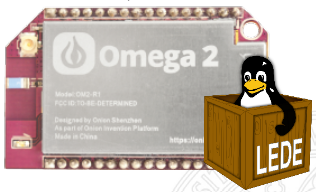
\includegraphics[width=\linewidth]{gfx/Omega2}
	
	Onion Omega2
} A device that falls inside the second category of IoT, powerful enough to run a familiar Linux environment, where we can develop and debug the first \acp{PoC} without troubling ourselves with non-related to the project problems.

Nonetheless, the Omega2 needs fine tunning to start operating, and basic knowledge of electronics is vital to make it work. The two main things to begin with Omega2 are:
\begin{itemize}
	\item A reliable 3.3V with a maximum of 800mA power supply (a USB with a step-down circuit works fine), with quality soldering and wires to avoid unwanted resistances.
	\item A Serial to USB adapter wired to the TX and RX UART pins to use the Serial Terminal, in case WiFi doesn't work and no SSH is available, and because the connection is more reliable in case of wireless interferences.
\end{itemize}


\begin{table}[h]
	\myfloatalign
	\begin{tabularx}{0.75\textwidth}{ll} \toprule
		MCU & Mediatek MT688 \citep{MT7688} \\
		CPU & MIPS32 24KEc 580MHz \\
		RAM & 64MB \\
		Storage & 16MB \\
		Firmware & LEDE (OpenWRT fork distro) \\
		Connectivity & Wifi b/g/n \\
		Power & 3.3V 300mA \\
		\bottomrule
	\end{tabularx}
	\caption[Onion Omega 2 Specifications]{Onion Omega2 Specifications.}
	\label{tab:Omega2Specs}
\end{table}




\paragraph{Raspberry Pi 3:}\marginpar{
	\vskip0pt
	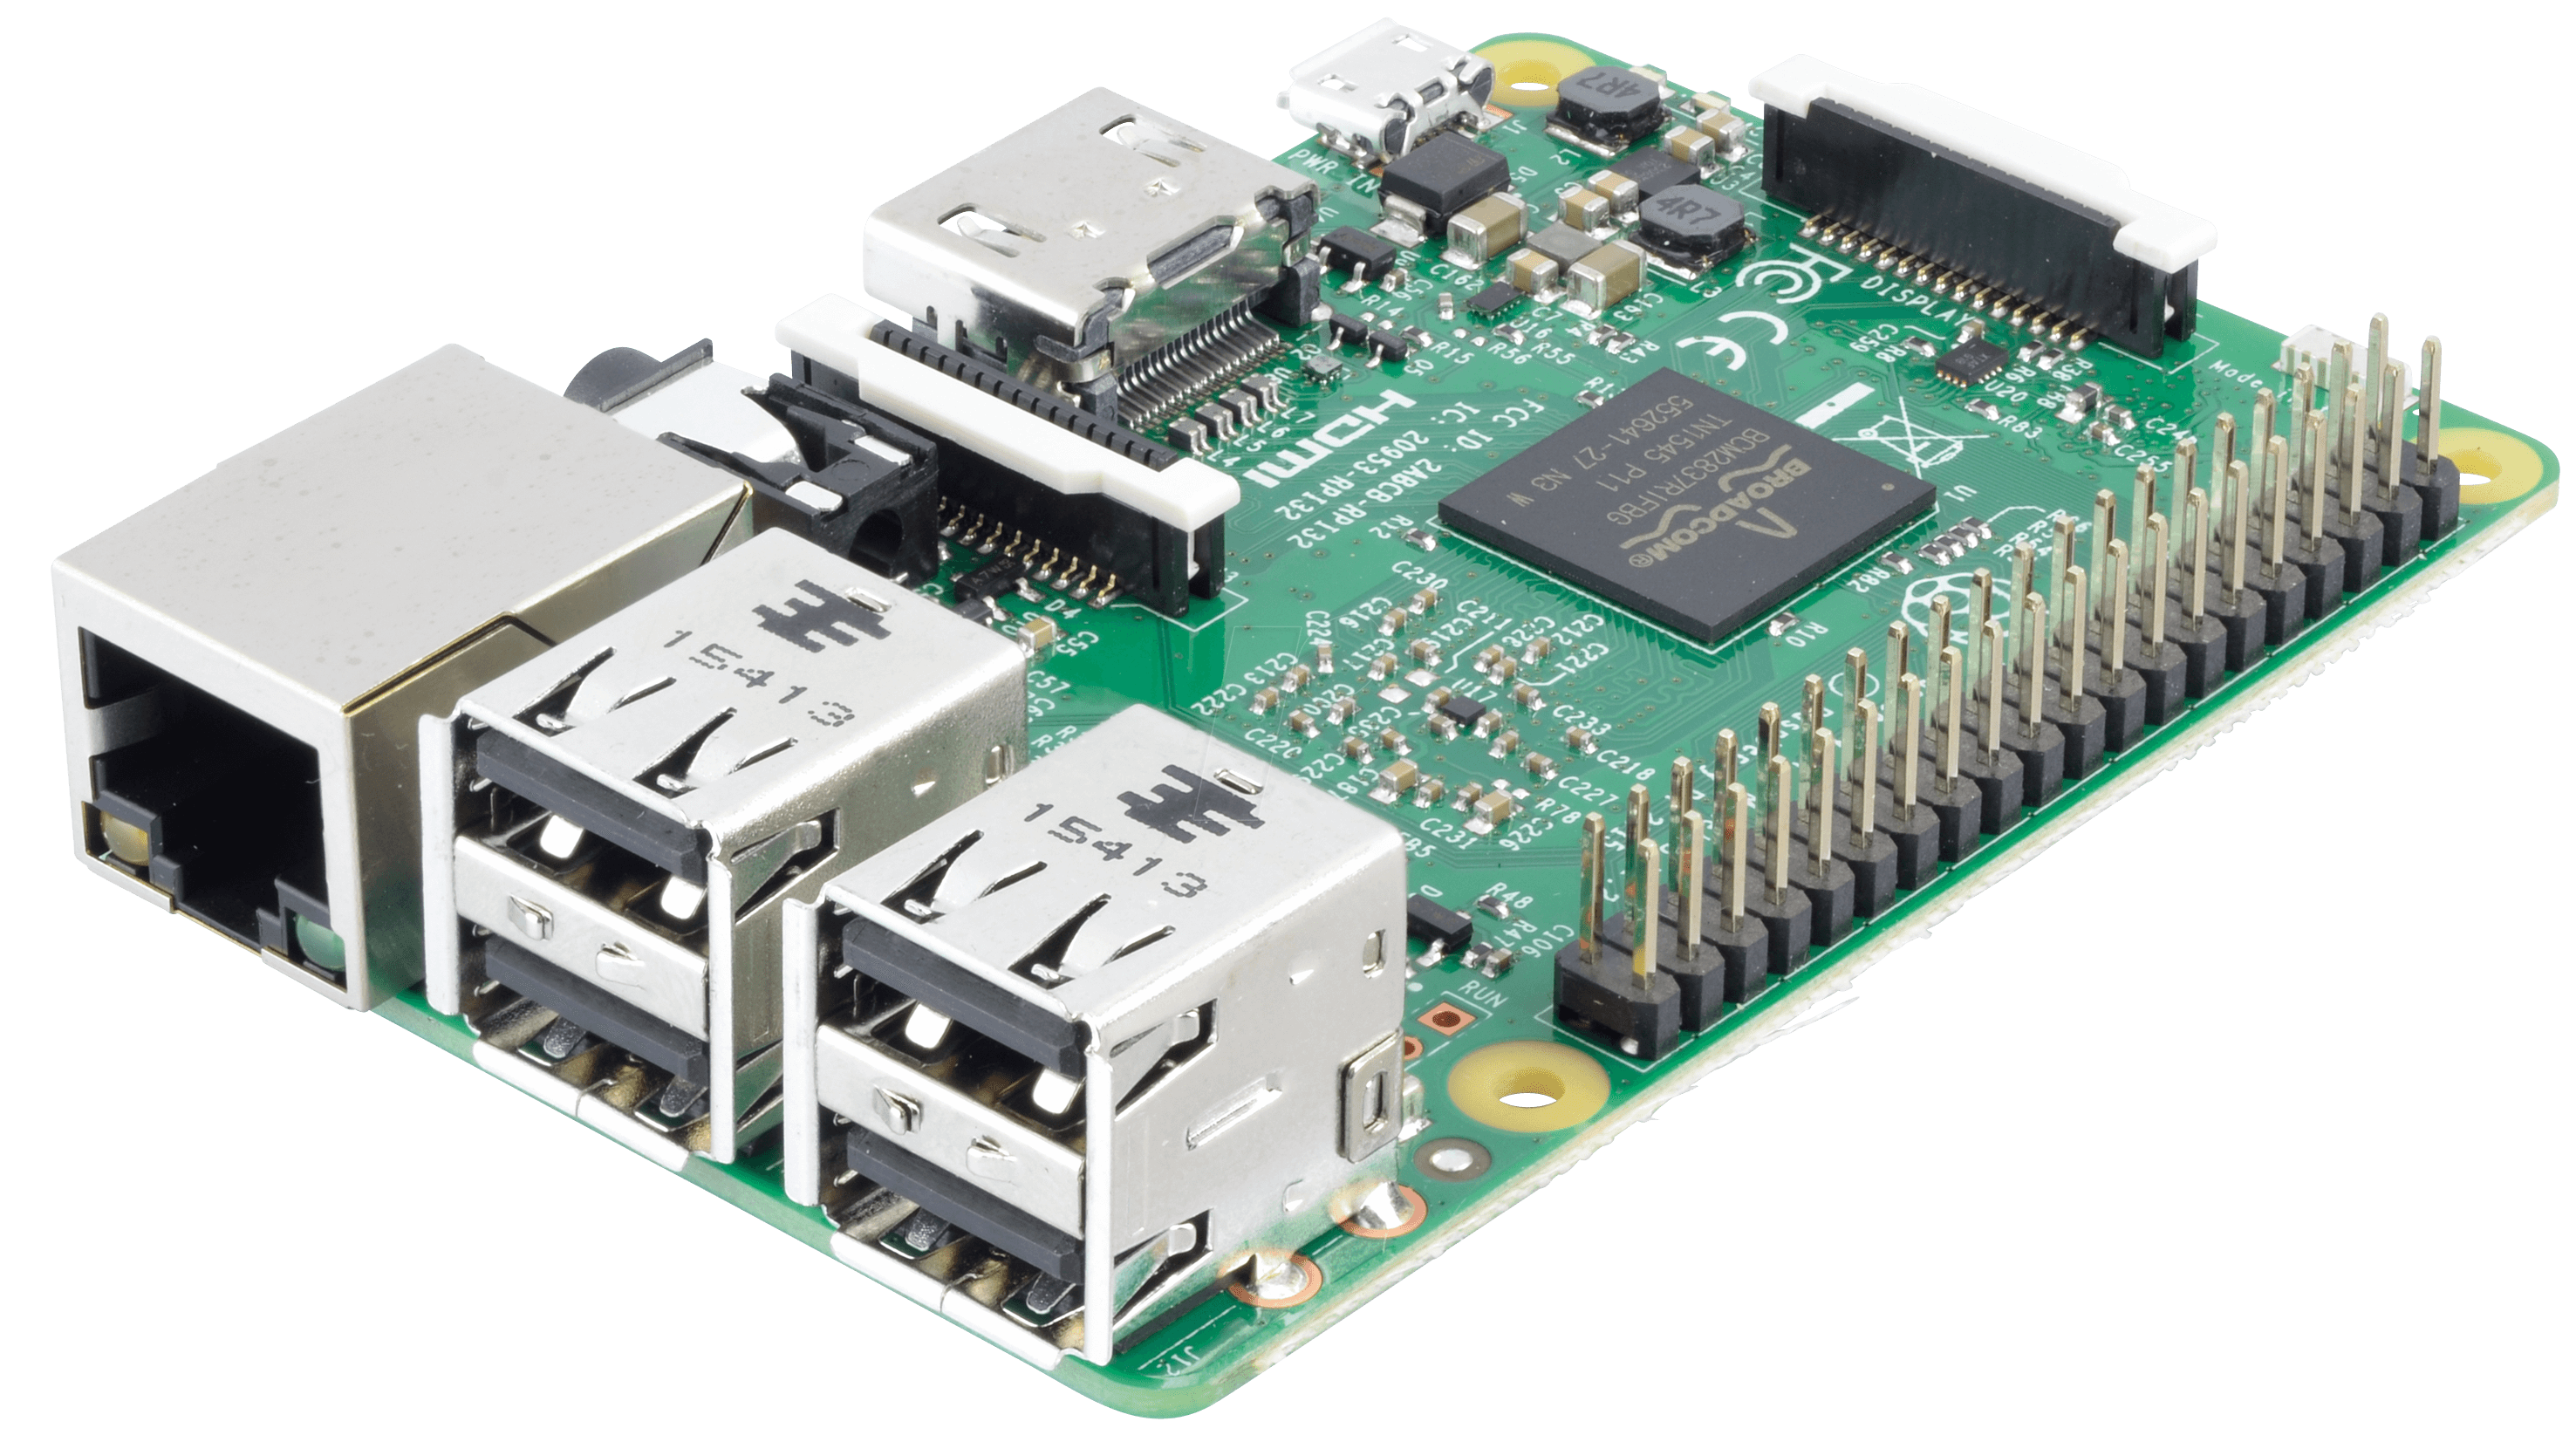
\includegraphics[width=\linewidth]{gfx/RPi3}
	
	Raspberry Pi 3
} Another familiar environment, powerful enough to debug and hold the delegated \ac{P2ABCE} Java services (User, Verifier, \dots) of P2ABC with its 1GB of RAM, and with two network interfaces it's perfect to work as the gateway for the IoT devices to the Internet.

Only a microSD with enough space to burn the binary with the OS is needed to plug\&play with the Raspberry Pi. We use Raspbian, a stable Debian based distro, recommended by the Raspberry Pi designers, and ready to use with the \ac{P2ABCE} compiled \textit{.jar} services.

\begin{table}[h]
	\myfloatalign
	\begin{tabularx}{0.75\textwidth}{ll} \toprule
		CPU & ARMv8 64bit quad-core 1.2GHz \\
		RAM & 1GB \\
		Storage & microSD \\
		Firmware & Raspbian (Debian based distro) \\
		Connectivity & Wifi n + Ethernet \\
		Power & 5V 2A \\
		\bottomrule
	\end{tabularx}
	\caption[Raspberry Pi 3 Specifications]{Raspberry Pi 3 Specifications.}
	\label{tab:RPi3Specs}
\end{table}





% C as pure as possible aiming to lower powerful devices without C++ support or std libraries
% LibGMP and OpenSSL for PoC
% CMake for portability and easy to config cross-compilation
% Java for P2ABCE
% Docker for building environments, both maven and LEDE SDK

\subsection{Software}

The development is divided between the \ac{IoT} device code and the \ac{P2ABCE} services.

\hfil

The P2ABCE is already written in Java, and few modifications will be done to the code in comparison to the existing project size, so we will continue using Java with the P2ABCE part.

\hfil

All IoT devices, have a C cross-compiler, some even a C++ cross-compiler. The worst case scenario is that one must write assembly code, and that code will be specific of that target, so we won't consider them.
If now we focus on the most constrained devices, we could find out that some can't compile C++, some may not have many common libraries, and that the memory limitations they face make practically impossible to use dynamic memory, if we want to avoid very possible execution malfunctions.

For that reason, the developed code for IoT devices must be written with standard C without using dynamic memory.

\hfil

A project with thousands of lines of code can't be written in a single file. And to manage the compilation of multiple files, organized in various directories, we will use CMake.

CMake has many advantages over Makefiles:

\begin{itemize}
	\item Cross-platform. It works in many systems, and more specifically, in Linux it generates Makefiles.
	\item Simpler syntax. Adding a library, files to compile, set definitions, etc. can be done with one CMake command, with rich documentation on the project's \href{https://cmake.org/cmake/help/latest/}{website}.
	\item Cross-compilation. With only a \href{http://www.vtk.org/Wiki/CMake_Cross_Compiling#The_toolchain_file}{\small{CMAKE TOOLCHAIN}} file, CMake sets up automatically the cross-compilation with Makefiles and the C/C++ cross-compiler provided.
\end{itemize}


\hfil

Although the ideal final code is pure C without external libraries or dynamic memory, the \ac{PoC} uses three major libraries:

\begin{itemize}
	\item OpenSSL: Provides reliable and tested AES and SHA256 implementations.
	\item LibGMP: Provides multiprecision integer modular arithmetic.
	\item cJSON: Provides a JSON parser to store and read the status in a human readable way.
\end{itemize}

These three libraries are used to implement different interfaces in the project, and C implementations of these interfaces should replace the external libraries in the future.

\hfil

Finally, we use Docker to deploy the compilation environments:

\paragraph{P2ABCE environment} A container with OpenJDK 7 and Maven installed, with the Idemix maven plugins installed following the project \href{https://github.com/p2abcengine/p2abcengine/wiki/How-to-Build-the-ABC-Engine}{instructions} to use Idemix as the Engine for P2ABCE.

\paragraph{LEDE SDK environment} A container with CMake and the LEDE SDK \citep{ledeproject} installed and configured for the Omega2 target.

The Dockerfiles can be found in the Appendix.
%TODO
%\include{multiToC} % <--- just debug stuff, ignore for your documents
% ********************************************************************
% Backmatter
%*******************************************************
\appendix
%\renewcommand{\thechapter}{\alph{chapter}}
\cleardoublepage
\part*{Appendix}
%********************************************************************
% Appendix
%*******************************************************
% If problems with the headers: get headings in appendix etc. right
%\markboth{\spacedlowsmallcaps{Appendix}}{\spacedlowsmallcaps{Appendix}}



\chapter{Test: APDU Commands exchanged}\label{ch:resultsdiagrams}


In this appendix we provide 3 sequence diagrams highlighting the APDU Commands exchanged during our testbed. 


The first one is the setup of the IoT smart card, storing the system parameters needed to work in the deployed P2ABCE system. The first Command is called \texttt{isAndroid} because the \texttt{HardwareSmartcard} class distinguishes Android phones acting as smart cards from MULTOS smart cards, in order to use Extended APDUs. Then configures the smart card, setting the PIN (``\texttt{1234}'' by default) and PUK. Finally, it copies the cryptographic system parameters to the smart card with multiple \texttt{SET} instructions.

The second image shows the issuance of the credential, divided in the three REST calls needed during the delegation. If we recall Idemix's issuance protocol, the User performed, during his first step, an exponentiation with his secret key and a ZKP, which can be identified by the \texttt{COMMITMENT} and \texttt{ISSUANCE RESPONSE} commands. During the second step, the User only has to verify the Issuer's ZKP and store the credential if the signature is valid. Because the P2ABC Engine can perform Verification of ZKP without the need of secret keys stored in the smart card, the APDU Commands in this phase are only for storing the credential information inside the IoT smart card's BLOB\footnote{\textbf{B}inary \textbf{L}arge \textbf{Ob}jects} database, with the \texttt{STORE BLOB} instruction. 


The last diagram represents the proving for the Presentation Policy received from a Verifier, using two REST calls. During the first REST call, the Service stores data for the proving in the smart card, but before starting the proving itself, the device must choose an identity for the proving. This is done with the Identity Service, that in the PoC chooses the first identity available. After this, the second REST call starts the proving, creating the \textit{commitment} and \textit{responses} that integrate any ZKP, and depends on the device's secret keys\footnote{We, again, refer the reader who wants to know more about ZKPs to \citep{tfgmates}.}.


\begin{figure}[bth]
	\begin{center}
		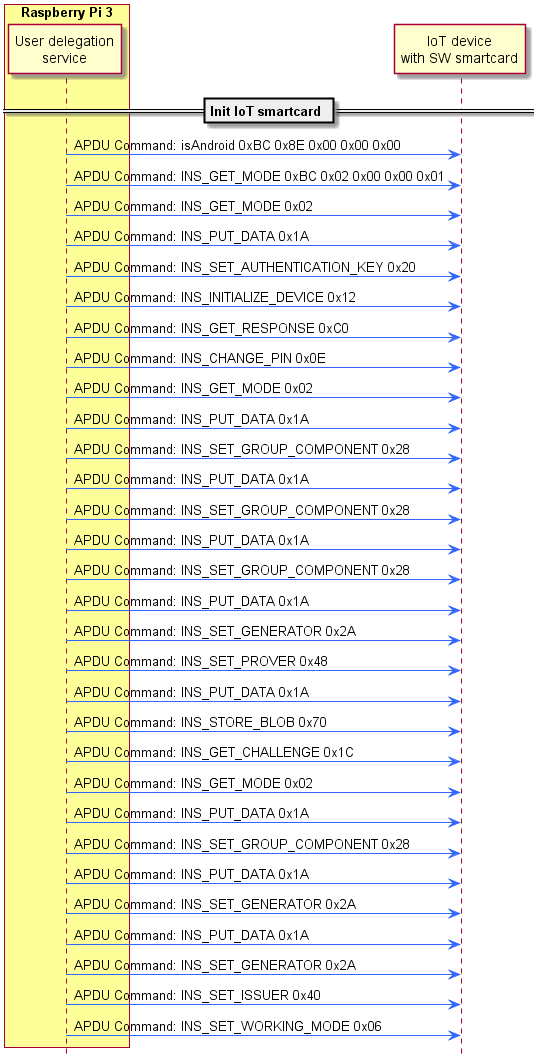
\includegraphics[width=0.9\linewidth]{gfx/UML/APDUsInitIoTSC}
	\end{center}
	\caption{Init IoT Smart Card APDU Commands exchanged.}
	\label{fig:APDUsInitIoTSC}
\end{figure}

\begin{figure}[bth]
	\begin{center}
		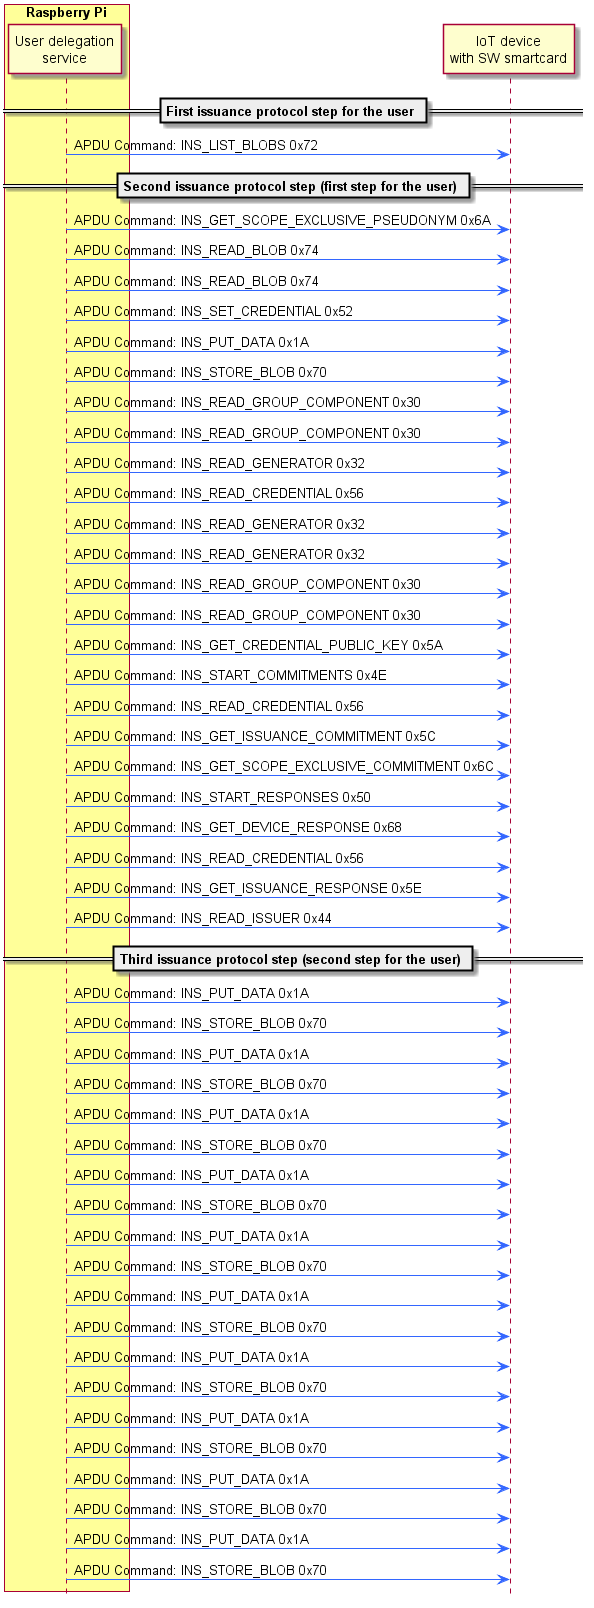
\includegraphics[width=0.78\linewidth]{gfx/UML/IssuanceAPDUs}
	\end{center}
	\caption{Issuance APDU Commands.}
	\label{fig:IssuanceAPDUs}
\end{figure}

\begin{figure}[bth]
	\begin{center}
		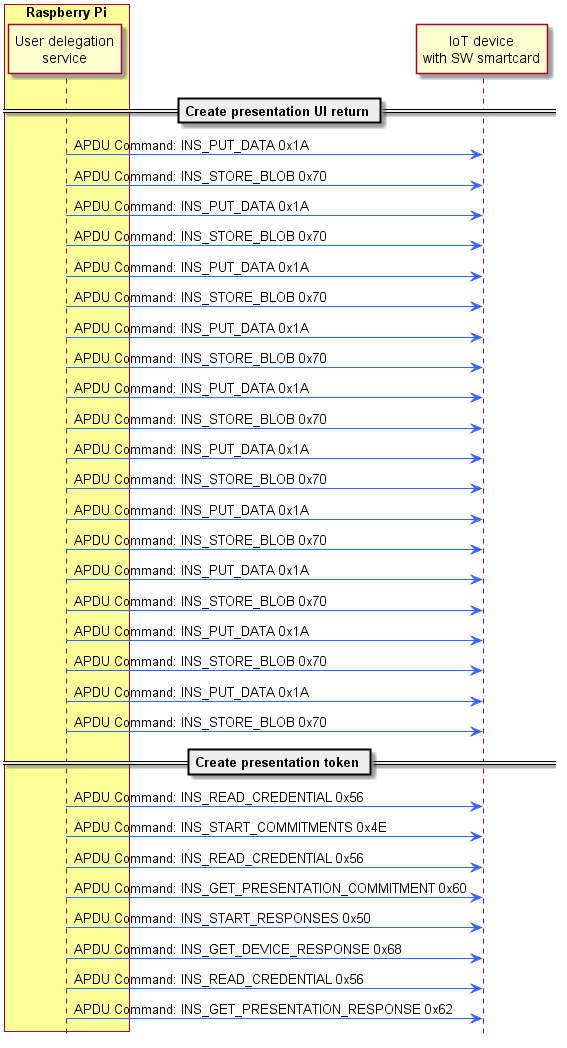
\includegraphics[width=\linewidth]{gfx/UML/APDUsProving}
	\end{center}
	\caption{Proving APDU Commands.}
	\label{fig:APDUsProving}
\end{figure}



\chapter{Paper proposal for JCR Magazine}\label{ch:JCR}

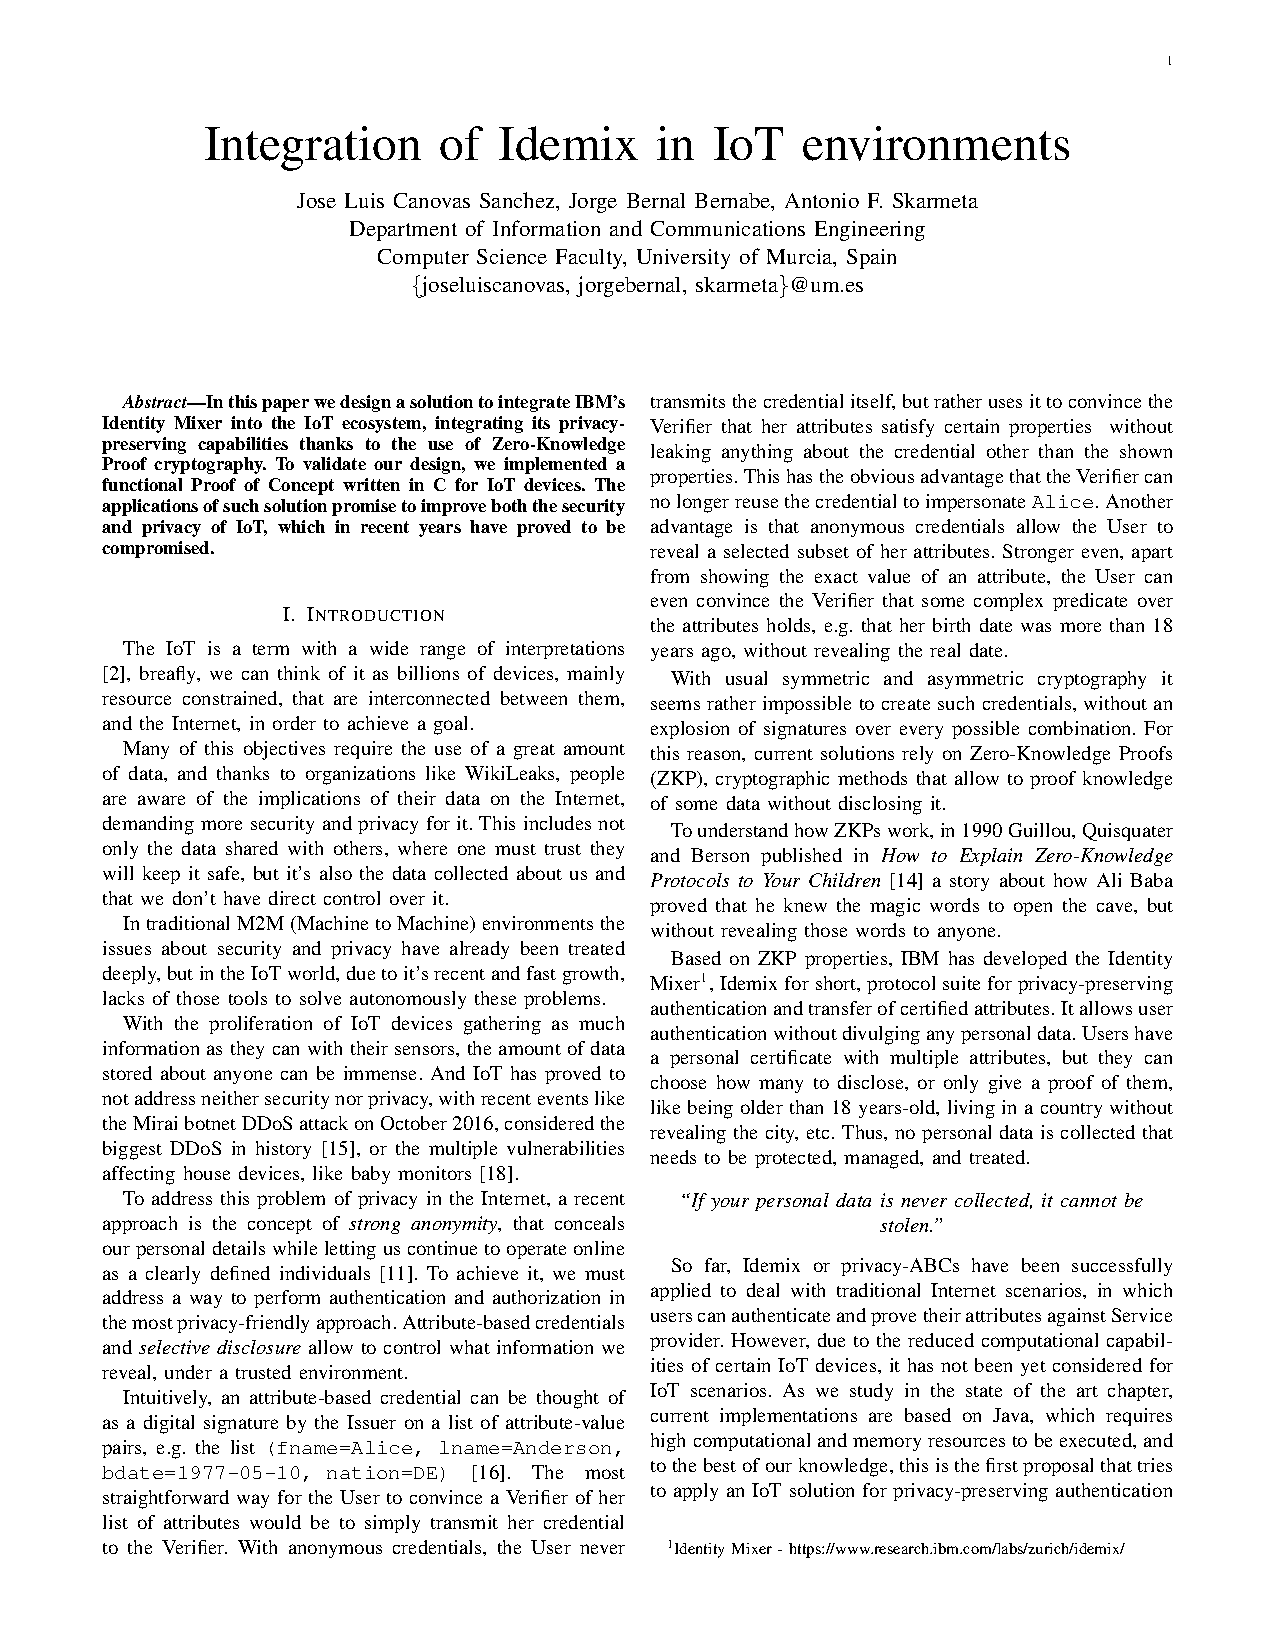
\includepdf[pages=-]{Chapters/bare_jrnl.pdf}


\chapter{Project's code structure}\label{ch:code}

Given the size of the project, we identify four main directory structures to arrange the code.


First, the Dockerfiles, scripts that automatize the creation of Docker images. These images are like virtual machine snapshots, although Docker is not a virtualization system, and we use the images to create containers, that are like new virtual machines started from the snapshots. We use two Dockerfiles, one for the P2ABCE compilation environment, with Java and Maven, and another one for building the Omega2 binaries, using the LEDE SDK.


\dirtree{%
	.1 Docker/. 
	.2 P2ABCE/. 
	.3 Dockerfile. 
	.3 idemix-3.0.36-binaries/. 
	.2 LEDE SDK/. 
	.3 Dockerfile. 
}

\hfil

The original P2ABCE project is of considerable size, but we list here the most interesting directories that we had to modify to make the project compatible with IoT smart cards.

\hfil

\dirtree{%
	.1 P2ABCE/. 
	.2 Code/. 
	.3 core-abce/. 
	.4 abce-components/. 
	.5 src/main/java/eu/abc4trust/smartcard/. 
	.6 IoTsmartcardio/.
	.7 util/. 
	.8 IoTsmartcardConnection.java.  
	.7 IoTCard.java. 
	.7 IoTCardChannel.java. 
	.7 IoTCardTerminal.java. 
	.6 HardwareSmartcard.java. 
	.6 SoftwareSmartcard.java. 
	.4 abce-services/. 
	.5 src/main/java/eu/abc4trust/services/. 
	.6 UserService.java. 
	.6 VerificationService.java. 
	.6 IssuanceService.java. 
}



\hfil

The IoT smart card toolkit is the core of this project. Managed with CMake, we see the \texttt{CMakeLists.txt} files, including the \texttt{Toolchain-omega2-mipsel.cmake} file with the cross-compiler information. We divide the project between the \textit{source} C files, and the header C files. Inside these directories, the organization is as stated in the implementation chapter: \textit{core} or \textit{common}, \textit{util interfaces} and \textit{external utilities}.

\hfil

\dirtree{%
	.1 p2abce\_iot\_toolkit/. 
	.2 CMakeLists.txt. 
	.2 Toolchain-omega2-mipsel.cmake. 
	.2 util\_sc\_tests/. 
	.2 util\_sc/. 
	.3 CMakeLists.txt. 
	.3 BIOSC.c. 
	.3 p2abc\_iot\_toolkit\_src/. 
	.4 smartcard\_common/. 
	.5 APDU\_handler.c. 
	.5 global\_vars.c. 
	.5 m\_adapted\_API.c. 
	.5 subroutines.c. 
	.4 smartcard\_external\_utilities/. 
	.5 cJSON.c. 
	.4 smartcard\_utils\_interface/. 
	.5 APDU\_IO\_util.c. 
	.5 arithmetic\_util.c. 
	.5 crypto\_util.c. 
	.5 serialize\_util.c. 
	.5 system\_funcs.c. 
	.3 p2abc\_iot\_toolkit\_include/. 
	.4 error\_codes.h. 
	.4 macrologger.h. 
	.4 smartcard\_common/. 
	.5 APDU\_handler.h. 
	.5 APDU\_types.h. 
	.5 abc4T\_types.h. 
	.5 defs\_consts.h. 
	.5 defs\_errs.h. 
	.5 defs\_ins.h. 
	.5 defs\_types.h. 
	.5 global\_vars.h. 
	.5 m\_adapted\_API.h. 
	.5 subroutines.h. 
	.4 smartcard\_external\_utilities/. 
	.5 base64.h. 
	.5 cJSON.h. 
	.4 smartcard\_utils\_interface/. 
	.5 APDU\_IO\_util.h. 
	.5 arithmetic\_util.h. 
	.5 crypto\_util.h. 
	.5 serialize\_util.h. 
	.5 system\_funcs.h. 
}


\hfil

Finally, the test scripts, including a Python file to test the BIOSC protocol, a directory with the testbed scripts (one file to orchestrate every device from one terminal), and a more didactic version with a script per device.

\hfil

\dirtree{%
	.1 scripts/. 
	.2 testBIOSC.py. 
	.2 tests/\DTcomment{One test script}. 
	.3 setupTest.sh. 
	.3 testNoIoT.sh. 
	.3 IoTtest.sh. 
	.2 distributed-PoC/\DTcomment{Distributed test}. 
	.3 Omega2/. 
	.3 RaspberryPi3/. 
	.3 ThirdPartyServer/. 
}
%********************************************************************
% Other Stuff in the Back
%*******************************************************
\cleardoublepage%********************************************************************
% Bibliography
%*******************************************************
% work-around to have small caps also here in the headline
\manualmark
\markboth{\spacedlowsmallcaps{\bibname}}{\spacedlowsmallcaps{\bibname}} % work-around to have small caps also
%\phantomsection 
\refstepcounter{dummy}
\addtocontents{toc}{\protect\vspace{\beforebibskip}} % to have the bib a bit from the rest in the toc
\addcontentsline{toc}{chapter}{\tocEntry{\bibname}}
\label{app:bibliography}
\printbibliography


\cleardoublepage%*******************************************************
% Declaration
%*******************************************************
\refstepcounter{dummy}
\pdfbookmark[0]{Declaration}{declaration}
\chapter*{Declaration}
\thispagestyle{empty}
Put your declaration here.
\bigskip
 
\noindent\textit{\myLocation, \myTime}

\smallskip

\begin{flushright}
    \begin{tabular}{m{5cm}}
        \\ \hline
        \centering\myName \\
    \end{tabular}
\end{flushright}

\cleardoublepage\pagestyle{empty}

\hfill

\vfill


\pdfbookmark[0]{Colophon}{colophon}
\section*{Colophon}
This document was typeset using the typographical look-and-feel \texttt{classicthesis} developed by Andr\'e Miede. 
The style was inspired by Robert Bringhurst's seminal book on typography ``\emph{The Elements of Typographic Style}''. 
\texttt{classicthesis} is available for both \LaTeX\ and \mLyX: 
\begin{center}
\url{https://bitbucket.org/amiede/classicthesis/}
\end{center}
Happy users of \texttt{classicthesis} usually send a real postcard to the author, a collection of postcards received so far is featured here: 
\begin{center}
\url{http://postcards.miede.de/}
\end{center}
 
\bigskip

\noindent\finalVersionString

%Hermann Zapf's \emph{Palatino} and \emph{Euler} type faces (Type~1 PostScript fonts \emph{URW
%Palladio L} and \emph{FPL}) are used. The ``typewriter'' text is typeset in \emph{Bera Mono}, 
%originally developed by Bitstream, Inc. as ``Bitstream Vera''. (Type~1 PostScript fonts were made 
%available by Malte Rosenau and
%Ulrich Dirr.)

%\paragraph{note:} The custom size of the textblock was calculated
%using the directions given by Mr. Bringhurst (pages 26--29 and
%175/176). 10~pt Palatino needs  133.21~pt for the string
%``abcdefghijklmnopqrstuvwxyz''. This yields a good line length between
%24--26~pc (288--312~pt). Using a ``\emph{double square textblock}''
%with a 1:2 ratio this results in a textblock of 312:624~pt (which
%includes the headline in this design). A good alternative would be the
%``\emph{golden section textblock}'' with a ratio of 1:1.62, here
%312:505.44~pt. For comparison, \texttt{DIV9} of the \texttt{typearea}
%package results in a line length of 389~pt (32.4~pc), which is by far
%too long. However, this information will only be of interest for
%hardcore pseudo-typographers like me.%
%
%To make your own calculations, use the following commands and look up
%the corresponding lengths in the book:
%\begin{verbatim}
%    \settowidth{\abcd}{abcdefghijklmnopqrstuvwxyz}
%    \the\abcd\ % prints the value of the length
%\end{verbatim}
%Please see the file \texttt{classicthesis.sty} for some precalculated 
%values for Palatino and Minion.
%
%    \settowidth{\abcd}{abcdefghijklmnopqrstuvwxyz}
%    \the\abcd\ % prints the value of the length





% ********************************************************************
% Game Over: Restore, Restart, or Quit?
%*******************************************************
\end{document}
% ********************************************************************
